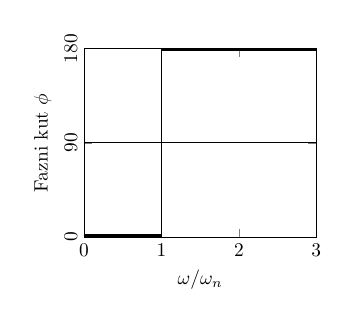
\begin{tikzpicture}[scale=0.7]
	\begin{axis} [
		height=5cm,
		ylabel = Fazni kut $\phi$, 
		xlabel = $\omega/\omega_n$,
		xmin = 0, xmax = 3,
		ymin = 0, ymax = 180,
		xtick = {0,1,2,3}, 
		ytick = {0,90,180}, yticklabel style={rotate=90},
	]
            \draw[thin] (0,90) -- (3,90);
            \draw[thin] (1,0)  -- (1,180);

        \addplot [
            domain=0:1,
            samples=200,
            color=black,
            line width=1mm,
        ]{atan((2*x*0)/(1-x^2))};
        \addplot [
                    domain=1.001:3,
                    samples=200,
                    color=black,
                    line width=1mm, 
       ]{180+atan((2*x*0)/(1-x^2))};
        \end{axis} 
\end{tikzpicture}
